\documentclass[16pt]{beamer}

\usetheme{default}
\usecolortheme{seagull}
\usefonttheme{structurebold}
\beamertemplatenavigationsymbolsempty
\setbeamertemplate{frametitle}[default][center]
\setbeamertemplate{footline}[frame number]

\AtBeginSection[]{
{
\setbeamercolor{background canvas}{bg=lightgray}
  \begin{frame}
  \vfill
  \centering
  \begin{beamercolorbox}[sep=8pt,center,shadow=true,rounded=true]{title}
    \usebeamerfont{title}\insertsectionhead\par%
  \end{beamercolorbox}
  \vfill
  \end{frame}
  }
}
   
%%%
% Packages
\usepackage{mathptm}
\usepackage{graphicx}
\usepackage{tikz}
%%%

%%%
% Marcos
\newenvironment{variableblock}[3]{%
\setbeamercolor{block body}{#2}
\setbeamercolor{block title}{#3}
\begin{block}{#1}}{\end{block}}
%%%

%%%
% Colors
\definecolor{bostonuniversityred}{rgb}{0.8, 0.0, 0.0}
\definecolor{etonblue}{rgb}{0.59, 0.78, 0.64}
\definecolor{grannysmithapple}{rgb}{0.66, 0.89, 0.63}
\definecolor{harvardcrimson}{rgb}{0.79, 0.0, 0.09}
\definecolor{lightapricot}{rgb}{0.99, 0.84, 0.69}
\definecolor{lightblue}{rgb}{0.68, 0.85, 0.9}
\definecolor{lightgray}{rgb}{0.83, 0.83, 0.83}

%%%

%%%
% Title page
\title{{}\\Title of the talk}
\author{{\large Borjan Geshkovski}}

\institute{
\begin{columns}
\begin{column}{0.65\textwidth}
   Joint work with:\\
\vspace*{0.1cm}
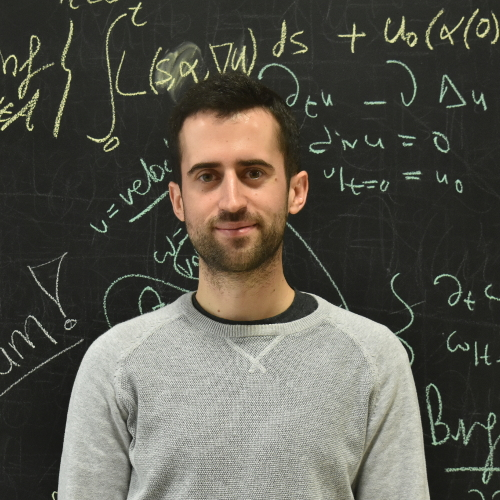
\includegraphics[scale=0.5]{figures/people/carlos}
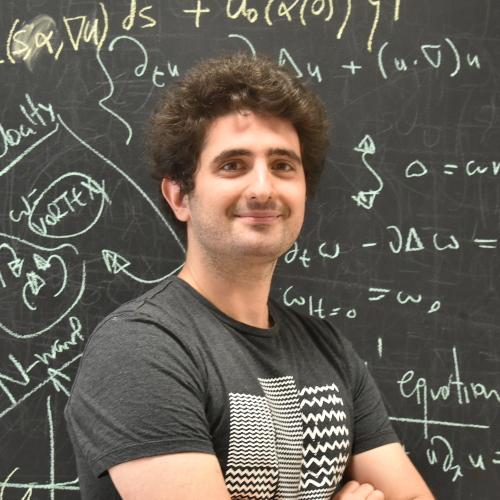
\includegraphics[scale=0.5]{figures/people/drb}\\
C. Esteve-Yag\"ue \hspace{0.1cm} D. Ruiz-Balet\\
(Cambridge) \hspace{0.45cm} (Imperial College)
\end{column}
\begin{column}{0.35\textwidth}  %%<--- here
    \begin{center}
    \vspace{4.75cm}
     
\includegraphics[scale=0.2]{figures/mit_logo}
     \end{center}
\end{column}
\end{columns}
}

% Date
\date{}
%%%

\begin{document}

% W background image
%{
%\usebackgroundtemplate{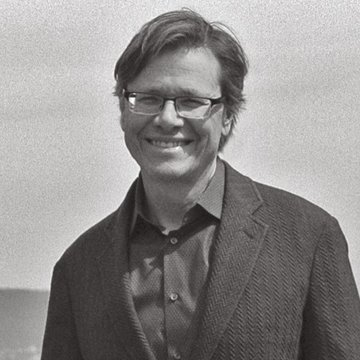
\includegraphics[width=\paperwidth]{figures/people/donoho}}
%\begin{frame}[noframenumbering, plain]
%\titlepage
%\end{frame}
%}

% No background image
\begin{frame}[noframenumbering, plain]
\titlepage
\end{frame}

\begin{frame}
\frametitle{Title of the slide}
This is some text in the first frame. This is some text in the first frame. This is some text in the first frame.

\begin{block}{Theorem}
The following holds true.
\end{block}
\end{frame}

\section{Section}

\begin{frame}
\frametitle{Another frame}

\begin{variableblock}{}{bg=grannysmithapple,fg=black}{bg=grannysmithapple,fg=white}
Stuff?
\end{variableblock}

\begin{columns}
\begin{column}{0.6\textwidth}
\begin{variableblock}{}{bg=lightapricot,fg=black}{bg=lightapricot,fg=white}
Stuff?
\end{variableblock}
\end{column}

\begin{column}{0.4\textwidth}
\begin{variableblock}{}{bg=lightblue,fg=black}{bg=lightblue,fg=white}
Stuff?
\end{variableblock}
\end{column}

\end{columns}


\end{frame}

\end{document}